\newpage
\section{柱函数}
\label{cylindrical}
\subsection{Bessel函数和Neumann函数}
在\nameref{Bessel}中,已经求得Bessel方程$x^2y''+xy'+(x^2-\nu^2)y=0$的基本解:

当$\nu\ne$整数时,Bessel方程的两个线性无关正则解为
$$
\boxed{\mathrm{J}_{\pm\nu}(x)=\sum_{k=0}^{\infty}\frac{(-1)^{k}}{k!\Gamma\left(k\pm\nu+1\right)}\left(\frac{x}{2}\right)^{2k\pm\nu}}
$$

其中$\Gamma(x)=\int_0^\infty e^{-t}t^{x-1}dt\quad,x>0$

当$\nu=n,n=0,1,2,3,...$时,$J_n,J_{-n}$不独立:$\mathrm{J}_{-n}(x)=(-1)^n\mathrm{J}_n(x)$

Bessel 方程的第一解仍是$J_\nu(x)$,第二解则可取为

\begin{dfn}[Neumann函数]
    $$\boxed{\mathrm{N}_\nu(x)=\frac{\cos\nu\pi\mathrm{J}_\nu(x)-\mathrm{J}_{-\nu}(x)}{\sin\nu\pi}}$$
\end{dfn}


$$\mathrm{N}_n(x)=\lim_{\nu\to n}\mathrm{N}_\nu(x)=\lim_{\nu\to n}\frac{\cos\nu\pi\mathrm{J}_\nu(x)-\mathrm{J}_{-\nu}(x)}{\sin\nu\pi}$$

应用 L'Hospital 法则,可得
$$\begin{aligned}
\mathrm{N}_n(x)=&\frac2\pi\mathrm{J}_n(x)\ln\frac x2-\frac1\pi\sum_{k=0}^{n-1}\frac{(n-k-1)!}{k!}\left(\frac x2\right)^{2k-n}\\
&-\frac1\pi\sum_{k=0}^\infty\frac{(-1)^k}{k!(k+n)!}\Big[\psi(n+k+1)+\psi(k+1)\Big]\Big(\frac x2\Big)^{2k+n}
\end{aligned}$$
$$\mathrm{N}_0(x)=\frac2\pi\mathrm{J}_0(x)\ln\frac x2
-\frac1\pi\sum_{k=0}^\infty\frac{(-1)^k}{(k!)^2}2\psi(k+1)\Big(\frac x2\Big)^{2k}$$

\begin{ex}
    $$\int_0^\infty\mathrm{e}^{-ax}\mathrm{J}_0(bx)\mathrm{~d}x\quad a>0$$
    代入 Bessel 函数的级数表示, 并逐项积分
    $$\begin{aligned}
        \int_0^\infty\mathrm{e}^{-ax}\mathrm{J}_0(bx) \mathrm{d}x& 
        =\int_0^\infty\mathrm{e}^{-ax}\sum_{k=0}^\infty\frac{(-1)^k}{(k!)^2}\left(\frac{bx}2\right)^{2k}\mathrm{d}x \\
        &=\sum_{k=0}^\infty\frac{(-1)^k}{(k!)^2}\left(\frac b2\right)^{2k} \int_0^\infty\mathrm{e}^{-ax}x^{2k} \mathrm{d}x \\
        &=\sum_{k=0}^\infty\frac{(-1)^k}{(k!)^2}\left(\frac b2\right)^{2k}\frac{(2k)!}{a^{2k+1}} \\
        &=\frac1a\sum_{k=0}^\infty\frac1{k!}\left(-\frac12\right)\left(-\frac32\right)\times\left(-\frac52\right)\cdots\left(-\frac{2k-1}2\right)\left(\frac ba\right)^{2k} \\
        &=\frac1a\left[1+\left(\frac ba\right)^2\right]^{-1/2}=\frac1{\sqrt{a^2+b^2}}
        \end{aligned}$$
\end{ex}

\subsubsection{递推关系}
$$\boxed{
    \begin{array}{c}
        \frac{\mathrm{d}}{\mathrm{d}x}\left[x^\nu\mathrm{J}_\nu(x)\right]=x^\nu\mathrm{J}_{\nu-1}(x)\\
        \frac{\mathrm{d}}{\mathrm{d}x}\left[x^{-\nu}\mathrm{J}_\nu(x)\right]=-x^{-\nu}\mathrm{J}_{\nu+1}(x)
    \end{array}}
    \quad
    \boxed{
    \begin{array}{c}
        \frac{\mathrm{d}}{\mathrm{d}x}\left[x^\nu\mathrm{N}_\nu(x)\right]=x^\nu\mathrm{N}_{\nu-1}(x)\\
        \frac{\mathrm{d}}{\mathrm{d}x}\left[x^{-\nu}\mathrm{N}_\nu(x)\right]=-x^{-\nu}\mathrm{N}_{\nu+1}(x)
    \end{array}}$$
    


\begin{prf}[递推关系1]
    $$\begin{aligned}
    \frac{d}{dx}(x^{\nu}J_{\nu})=&\frac{d}{dx}\left[\sum_{k=0}^{\infty}(-1)^{k}\frac{1}{k!\Gamma(k+\nu+1)}\frac{1}{2^{2k+\nu}}x^{2k+2\nu}\right]\\
    \mbox{逐项对}x\mbox{求导}\quad=&\sum_{k=0}^{\infty}\frac{(-1)^{k}}{k!\Gamma(\nu+k+1)}\frac{2(k+\nu)}{2^{2k+\nu}}x^{2k+2\nu-1}\\
    =&\sum_{k=0}^{\infty}(t)^{k}\frac{1}{k!\Gamma(\nu+k)}\left(\frac{x}{2}\right)^{2k+\nu-1}x^{\nu}\\
    =&x^\nu\mathrm{J}_{\nu-1}(x)
    \end{aligned}$$

\begin{rem}
由$\Gamma(x+1)=x\Gamma(x)$可得
$$\frac{k+\nu}{\Gamma(\nu+k+1)}=\frac{1}{\Gamma(\nu+k)}$$
\end{rem}
\end{prf}

\begin{prf}[递推关系2]
    $$\begin{aligned}
        \frac{\mathrm{d}}{\mathrm{d}x}\left[x^{-\nu}\mathrm{J}_\nu(x)\right]
        &=\frac{\mathrm{d}}{\mathrm{d}x}\sum_{k=0}^\infty\frac{(-1)^k}{k! \Gamma\left(k+\nu+1\right)}\frac{x^{2k}}{2^{2k+\nu}}\\
        &=\sum_{k=0}^\infty\frac{(-1)^{k+1}}{k! \Gamma\left(k+\nu+2\right)}\frac{x^{2k+1}}{2^{2k+\nu+1}}
        =-x^{-\nu}\mathrm{J}_{\nu+1}(x)
    \end{aligned}$$
\end{prf}

将此二递推关系写成
$$\nu x^{\nu-1}\mathrm{J}_\nu(x)+x^\nu\mathrm{J}_\nu^{\prime}(x)=x^\nu\mathrm{J}_{\nu-1}(x)$$
$$-\nu x^{-\nu-1}\mathrm{J}_\nu(x)+x^{-\nu}\mathrm{J}_\nu^{\prime}(x)=-x^{-\nu}\mathrm{J}_{\nu+1}(x)$$

消去$J_\nu(x)$或$J′_\nu(x)$, 又可以得到两个新的递推关系
$$\boxed{
    \begin{array}{c}
        \mathrm{J}_{\nu-1}(x)-\mathrm{J}_{\nu+1}(x)=2\mathrm{J}_\nu^{\prime}(x)\\
        \mathrm{J}_{\nu-1}(x)+\mathrm{J}_{\nu+1}(x)=\frac{2\nu}x\mathrm{J}_\nu(x)
    \end{array}}
    $$
\begin{ex}
    $$\int_0^1\left(1-x^2\right)\mathrm{J}_0(\mu x)x\mathrm{~d}x$$

    其中$\mu$是$J_0(x)$的零点,$J_0(\mu)=0$

由递推关系1,
$$
\frac1\mu\frac{\mathrm{d}}{\mathrm{d}x}\left[x\mathrm{J}_1(\mu x)\right]=x\mathrm{J}_{0}(\mu x)
$$

积分得

$$\begin{aligned}
&\int_0^1\left(1-x^2\right)\mathrm{J}_0(\mu x)x\mathrm{~d}x\\
=&\frac1\mu\int_0^1(1-x^2)\frac{\mathrm{d}}{\mathrm{d}x}\left[x\mathrm{J}_1(\mu x)\right]\mathrm{~d}x\\
\mbox{分部积分}\quad=&(1-x^2)\frac{1}{\mu}xJ_1(\mu x)\bigg|_0^1+\frac{2}{\mu}\int_0^1x^2J_1(\mu x)dx\\
\mbox{第一项为零,第二项继续使用递推关系1}\quad=&\frac{2}{\mu^2}\int_{0}^{1}\frac{d}{dx}[x^2J_2(\mu x)]dx\\
=&\frac{2}{\mu^2}x^2J_2(\mu x)\bigg|_0^1\\
=&\frac{2}{\mu^2}J_2(\mu)=\frac{4}{\mu^3}J_1(\mu)
\end{aligned}$$
\end{ex}

\begin{app}[幂函数乘Bessel函数积分]
    $$\begin{aligned}
    &\int_{a}^{b}x^{\mu}J_{\nu}(x)dx\\
    =&\int_{a}^{b}x^{\mu-\nu-1}x^{\nu+1}J_{\nu}dx=\int_{a}^{b}x^{\mu-\nu-1}\frac{d}{dx}[x^{\nu+1}J_{\nu+1}]dx\\
    =&x^{\mu-\nu-1}x^{\nu+1}J_{\nu+1}\bigg|_{a}^{b}-(\mu-\nu-1)\int_{a}^{b}x^{\mu-\nu-2}x^{\nu+1}J_{\nu+1}dx\\
    =&\dots\\
    =&
    \end{aligned}$$

两类易算情况

1. $(u-n)-(\nu+n)=1$,即$\mu-\nu=2n+1$ 
$$\int_{a}^{b}x^{\nu+n+1}J_{\nu+n}dx=\int_{a}^{b}\frac{d}{dx}[x^{\nu+n+1}J_{\nu+n+1}]dx$$

2. $(u-n)+(\nu+n)=1$,即$\mu+\nu=1$ 
$$\int_{a}^{b}x^{-(\nu+n-1)}J_{\nu+n}dx=\int_{a}^{b}\frac{d}{dx}[x^{-(\nu+n-1)}J_{\nu+n-1}]dx $$
\end{app}

\subsection{渐进行为}
\begin{figure}[htbp]
    \centering
    \begin{minipage}[t]{0.48\textwidth}
    \centering
    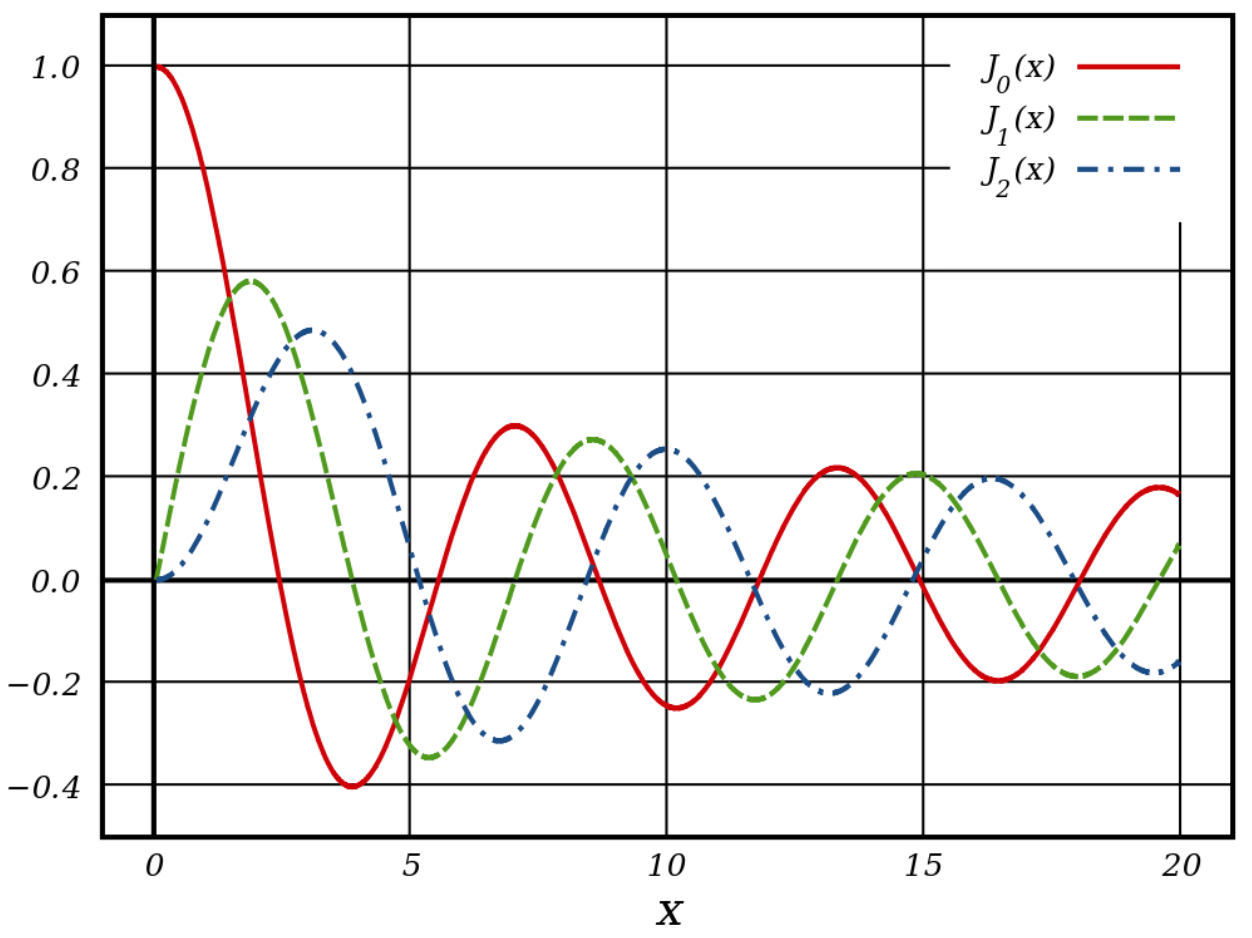
\includegraphics[width=7cm]{figures/BesselFunction.png}
    \caption{Bessel函数}
    \end{minipage}
    \begin{minipage}[t]{0.48\textwidth}
    \centering
    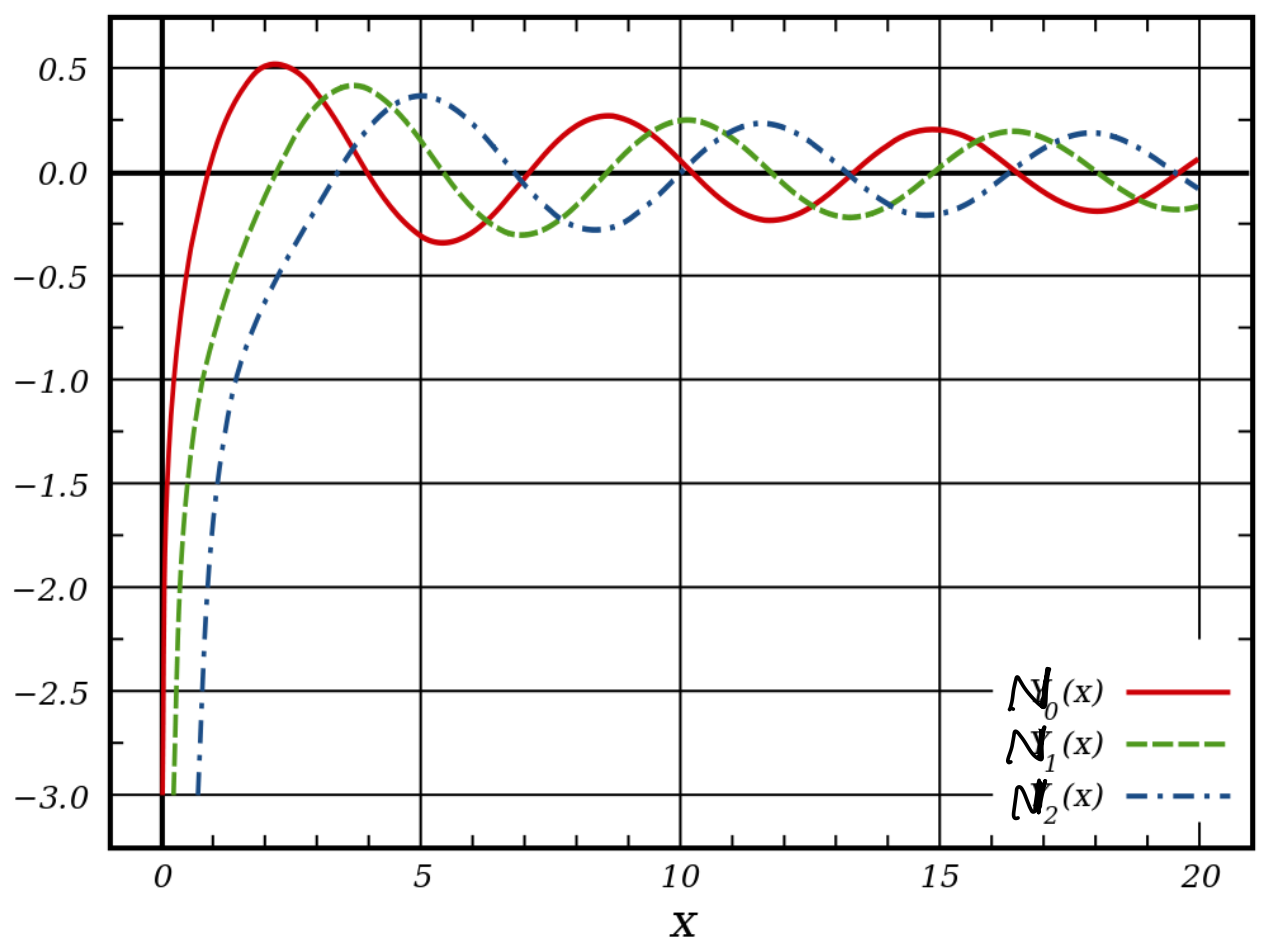
\includegraphics[width=7cm]{figures/NeumannFunction.png}
    \caption{Neumann函数}
    \end{minipage}
\end{figure}
\subsubsection{$x\rightarrow0$}
\noindent 1. Bessel函数
$$J_{\nu}(x)=
\sum_{k=0}^{\infty}(-1)^{k}\frac{1}{k!\Gamma(u+k+1)}\left(\frac{x}{2}\right)^{2k+\nu}
\quad (k=0\mbox{主导})\sim\frac{1}{\Gamma(\nu+1)}\left(\frac{x}{2}\right)^{\nu}
$$
$$
\begin{cases}\nu=0&J_{0}(x)\rightarrow1\\\nu>0&J_{\nu}(x)\sim\frac{1}{\Gamma(\nu+1)}(\frac{x}{2})^{2}\rightarrow0\end{cases}
$$
\noindent 2. Neumann函数

$$
\begin{cases}
    \nu=0&N_{0}(x)\rightarrow\infty\\
    \nu>0&J_{\nu}(x)\sim\frac{1}{\Gamma(\nu+1)}(\frac{x}{2})^{2}\rightarrow\infty
\end{cases}$$

$\nu>0$时:
$$\begin{aligned}
\mathrm{N}_\nu(x)=&\frac{\cos\nu\pi\mathrm{J}_\nu(x)-\mathrm{J}_{-\nu}(x)}{\sin\nu\pi}\\
(\mathrm{J}_{-\nu}\mbox{主导})\sim& -\frac{J_{-\nu}(x)}{\sin \nu\pi}\\
(k=0\mbox{主导})\sim& -\frac{1}{\sin \nu\pi}\frac{1}{\Gamma(1-\nu)}(\frac{x}{2})^{-u}\\
\left[\mbox{由}\Gamma(x)\Gamma(1-x)=\frac{\pi}{\sin\pi x}\right]\sim&-\frac{T(\nu)T(1-\nu)}{\pi}\frac{1}{\Gamma(1-\nu)}\left(\frac{x}{2}\right)^{-\nu}\\
\sim&-\frac{\Gamma(\nu)}{\pi}\left(\frac{x}{2}\right)^{-\nu}\rightarrow\infty
\end{aligned}$$

$\nu=0$时:
$$N_{0}(x)\sim\frac{2}{\pi}J_{0}(x)\ln\frac{x}{2}+\text{幂级数}\sim\frac{2}{\pi}\ln\frac{x}{2}\rightarrow\infty$$


\subsubsection{$x\rightarrow\infty$}
$$\begin{aligned}
    J_{\nu}(x)&\sim\sqrt{\frac{2}{\pi x}}\cos(x-\frac{\nu\pi}{2}-\frac{\pi}{4})\\
    N_{\nu}(x)&\sim\sqrt{\frac{2}{\pi x}}\sin(x-\frac{\nu\pi}{2}-\frac{\pi}{4})\end{aligned} \quad\text{振荡衰减}
$$

\noindent 0级近似:
$$y^{\prime\prime}+\frac{1}{x}y^{\prime}+(1-\frac{\nu^{2}f}{x^{2}})y=0\Rightarrow y^{\prime\prime}+y\approx0\Rightarrow y(x)\sim\cos(x-x_0)$$

\noindent 1级近似:待定$y(x)=f(x)\cos(x-x_0)$
$$y''+\frac{1}{x}y'+(1-\frac{\nu^2}{x^2})y=(f^{\prime}\cos-2f^{\prime}\sin-f\cos)+\frac{1}{x}(f^{\prime}\cos-f\sin)+(1-\frac{\nu^{2}}{x})f\cos=0$$
$$(f^{\prime\prime}\cos-2f^{\prime}\sin)+\frac{1}{x}(f^{\prime}\cos-f\sin)-\frac{\nu^{2}}{x^{2}}f\cos=0$$
$$-(2f^{\prime}+\frac{f}{x})\sin x+(f^{\prime\prime}+\frac{1}{x}f^{\prime}-\frac{\nu^{2}}{x^{2}}f)\cos x=0$$

$$\begin{aligned}
&\sin\text{系教}=0\Rightarrow 2f^{\prime}+\frac{f}{x}=0\Rightarrow f(x)\sim x^{-\frac{1}{2}}\\
&\cos\text{系数}f^{\prime\prime}+\frac{1}{x}f^{\prime}-\frac{\nu^{2}}{x^{2}}f\sim x^{-\frac{5}{2}},\text{是更高阶小量}
\end{aligned}$$

因此$y(x)\sim f(x)\cos(x-x_{0})\sim\sqrt{\frac{1}{x}}\cos(x-x_{0})$

\subsection{Bessel 函数的应用}
\begin{ex}[扩散问题]
    $$\frac{\partial u}{\partial t}=D\nabla^{2}u,r<a$$
    $$\begin{aligned}
        &u|_{\phi=0}=u|_{\phi=2\pi},&&\frac{\partial u}{\partial\phi}\bigg|_{\phi=0}=\frac{\partial u}{\partial\phi}\bigg|_{\phi=2\pi}\\
        &u|_{t=a}=0,\quad &&u|_{t=0}=f(r,\phi)
    \end{aligned}$$
\noindent 分离变量$u=V(r,\phi)T(t)$得
$$\frac{\nabla^{2}V}{V}=\frac{T^{\prime}}{DT}=-E$$

\noindent 时间上:$T^{\prime}=-DET$

\noindent 空间上:
$$\begin{cases}
    \nabla^{2}V+EV=\frac{1}{r}\frac{\partial}{\partial r}(r\frac{\partial V}{\partial r})+\frac{1}{r^{2}}\frac{\partial^{2}V}{\partial\phi^{2}}+EV=0,\\
    V|_{r=a}=0,V|_{r=0}<\infty\\
    V|_{\phi=0}=V|_{\phi=2\pi},\frac{\partial V}{\partial\phi}|_{\phi=0}=\frac{\partial V}{\partial\phi}|_{\phi=2\pi}
\end{cases}$$

\noindent 空间上,进一步分离变量:$V(r,\phi)=R(r)\Phi(\phi)$

角向
$$\begin{cases}
    \Phi^{\prime\prime}+\lambda\Phi=0\\
    \Phi(0)=\Phi(2\pi),\Phi^{\prime}(0)=\Phi^{\prime}(2\pi)
\end{cases}
\Rightarrow \lambda=m^2,\quad
\Phi_{m}=
\begin{cases}
    \cos m\phi&m=0,1,2\ldots\\
    \sin m\phi&m=1,2\ldots
\end{cases}$$

径向
$$\begin{cases}
    \frac{1}{r}\frac{d}{dr}(r\frac{dR}{dr})+(E-\frac{\lambda}{r^{2}})R=0\\
    R(0)<\infty,R(a)=0
\end{cases}$$

$$\begin{aligned}
(E=k^2) \quad &r\frac{d}{dr}(r\frac{dR}{dr})+(k^{2}r^{2}-m^{2})R=0\\
(x=kr) \quad &x\frac{d}{dx}(x\frac{dR}{dx})+(x^{2}-m^{2})R=0
\end{aligned}$$

$$x^{2}R''+xR^{\prime}+(x^{2}-m^{2})R=0$$
$$\Rightarrow R=CJ_{m}(x)+DN_{m}(x)$$

由于$R(0)<\infty, N_m(x)$项系数为零,
$$R=CJ_{m}(x)=CJ_{m}(kr)$$
$$R(a)=0\Rightarrow J_{m}(ka)=0\Rightarrow ka=\mu_{i}^{(m)}$$

其中$\mu_i$为$J_m(x)$的第$i$个正零点$(m=0,1,2,\dots;\quad i=1,2,3,\dots)$
$$k_{mi}=\frac{\mu_{i}^{(m)}}{a}$$

本征值
$$E_{mi}=\left(\frac{\mu_{i}^{(m)}}{a}\right)^{2}$$

径向本征函数
$$R_{mi}(r)=J_{m}(k_{mi}r)=J_{m}\left(\frac{\mu_{i}^{(m)}}{a}r\right)$$

V的本征函数$(i=1,2,3,\dots)$
$$\begin{cases}
    V_{mi1}=R_{mi}(r)\cos m\phi=J_{m}\left(\frac{\mu_{i}^{(m)}}{a}r\right)\cos m\phi&m=0,1,2,\dots\\
    V_{mi2}=R_{mi(r)}\sin m\phi=J_{m}\left(\frac{\mu_{i}^{(m)}}{a}r\right)\sin m\phi&m=1,2,3,\dots
\end{cases}$$

\noindent 得到一般解形式:
$$\begin{aligned}
u(r,\phi,t)=&\left(\sum_{m}\sum_{i}A_{mi}V_{mi1}+\sum_{m}\sum_{i}B_{mi}V_{mi2}\right)e^{-DE_{mi}t}\\
=&\left[\sum_{m=0}^{\infty}\sum_{i=1}^{\infty}A_{mi}R_{mi}(r)\cos m\phi+\sum_{m=1}^{\infty}\sum_{i=1}^{\infty}B_{mi}R_{mi}(r)\sin m\phi\right]e^{-DE_{mi}t}
\end{aligned}$$

\noindent 利用初始条件确定$A_{mi},B_{mi}$:
$$\begin{aligned}
u|_{t=0}=f(r,\phi)=&\sum_{m=0}^{\infty}\sum_{i=1}^{\infty}A_{mi}R_{mi}(r)\cos m\phi &&+\sum_{m=1}^{\infty}B_{mi}R_{mi}(r)\sin m\phi\\
f(r,\phi)=&\sum_{m=0}^{\infty}f_{m1}(r)\cos m\phi &&+\sum_{m=1}^{\infty}f_{m2}(r)\sin m\phi 
\end{aligned}$$

比较$\cos$和$\sin$的系数
$$f_{m1}(r)=\sum_{i=1}^{\infty}A_{m_{i}}R_{m_{i}}(r)=\sum_{i=1}^{\infty}A_{mi}-J_{m}\left(\frac{\mu_{i}^{(m)}}{a}r\right)$$
$$f_{m2}(r)=\sum_{i=1}^{\infty}B_{m_{i}}R_{m_{i}}(r)=\sum_{i=1}^{\infty}B_{mi}-J_{m}\left(\frac{\mu_{i}^{(m)}}{a}r\right)$$
即$f_{m1}(r),f_{m2}(r)$按$J_{m}\left(\dfrac{\mu_{i}^{(m)}}{a}r\right)$展开.

\noindent 由正交性确定系数:

将方程改写为S-L标准形式,可见$r$为权函数
$$\frac{d}{dr}\left(r\frac{dR}{dr}\right)+(k^{2}r-\frac{m^{2}}{r})R=0$$
$$R(0)<\infty,R(a)=0$$

可得正交性
$$\int_{a}^{b}J_{m}\left(\frac{\mu_{i}^{(m)}}{a}r\right)J_{m}\left(\frac{\mu_{j}^{(m)}}{a}r\right)rdr=0(i\neq j)$$

\noindent 广义傅里叶级数
$$\begin{aligned}
    [0,a]&=f(r)=\sum_{i=1}^{\infty}b_{i}J_{m}\left(\frac{\mu_{i}^{(m)}}{a}r\right)\\
    b_{i}&=\frac{1}{||J_{m}(\frac{\mu_{i}^{(m)}}{a}r)||^{2}}\int_{0}^{a}f(r)J_{m}\left(\frac{\mu_{i}^{(m)}}{a}r\right)rdr
\end{aligned}$$

模方

$$\boxed{
   \bigg|\bigg|J_{m}\left(\frac{\mu_{i}^{(m)}}{a}r\right)\bigg|\bigg|^{2}
    \equiv\int_{0}^{a}\left[J_{m}\left(\frac{\mu_{i}^{(m)}}{a}r\right)\right]^{2}rdr
    =\frac{a^{2}}{2}\left[J_{m+1}\left(\mu_{i}^{(m)}\right)\right]^{2}
}$$

计算过程:
$$\int_{0}^{a}[J_{m}(\frac{\mu_{i}^{(m)}}{a}r)]^{2}rdr\xlongequal{x=\frac{\mu_{i}^{(m)}}{a}r}\left(\frac{a}{\mu_{i}^{(m)}}\right)^{2}\int_{0}^{\mu_{i}^{(m)}}[J_{m}(x)]^{2}xdx$$

其中,
$$\begin{aligned}
    \int_{0}^{a}[J_{m}(x)]^{2}xdx
    =&\frac{a^{2}}{2}[J_{m}^{\prime}(a)]^{2}+\frac{1}{2}(a^{2}-m^{2})[J_{m}(a)]^{2},\quad m\geq0\\
    \xlongequal{\text{if\ }J_{m}(a)=0}&\frac{a^{2}}{2}[J_{m+1}(a)]^{2}
\end{aligned}$$
\end{ex}

\begin{ex}[Laplace方程:圆柱体内稳定温度分布]
    $$\begin{aligned}
        &\nabla^{2}u=0\quad r<a,\quad0<z<h\\
        &u|_{r=a}=0,\quad u|_{z=0}=0,u|_{z=h}=u_{0}
    \end{aligned}$$

\noindent 分离变量$u(r,z)=R(r)Z(z)$(对称性)
$$\nabla^{2}u=\frac{1}{r}\frac{\partial}{\partial r}(r\frac{\partial u}{\partial r})+\frac{\partial^2 u}{\partial z^{2}}=0$$

\noindent $r$方向解本征值问题
$$\begin{cases}
    (rR^{\prime})^{\prime}+\lambda rR=0\\
    R(0)<\infty,R(a)=0
\end{cases}$$

$$r^{2}R''+rR'+\lambda r^{2}R=0$$

变量代换$x=\sqrt{\lambda}r$,得到0阶Bessel方程形式
$$x^{2}\frac{d^{2}R}{dx^{2}}+x\frac{dR}{dx}+(x^{2}-0^{2})R=0$$

解得$r$方向本征函数的形式(由于$N_0(x)$在$x=0$发散,需要舍弃)
$$R=J_0(x)=J_0(\sqrt{\lambda}r)$$

利用边界条件求本征值,其中$\mu_i$为0阶Bessel方程的第$i$个正零点
$$R(a)=0\Rightarrow J_{0}(\sqrt{\lambda}a)=0\Rightarrow\lambda_{i}=(\frac{\mu_{i}}{a})^{2}$$

最终得到$r$方向本征函数
$$R_{i}(r)=J_{0}\left(\frac{\mu_{i}}{a}r\right)\quad i=1,2,3\ldots$$

\noindent $z$方向
$$z''-\lambda z=0$$
$$z_{i}(z)=A_{i}e^{\frac{\mu_{i}}{\alpha}z}+B_{i}e^{-\frac{\mu_{i}}{\alpha}z}$$

\noindent 一般解形式
$$u(r,z)=\sum_{i=1}^{\infty}R_{i}(r)Z_{i}(z)$$

$z=0$处边界条件:$u|_{z=0}=0\Rightarrow A_i+B_i=0$
$$u(r,z)=\sum_{i=1}^{\infty}C_{i}\sinh(\frac{\mu_{i}}{a}z)J_{0}(\frac{\mu_{i}}{a}r)$$

$z=h$处边界条件:
$$u|_{z=h}=u_{0}=\sum_{i=1}^{\infty}C_{i}\sinh\frac{\mu_{i}h}{a}J_{0}(\frac{\mu_{i}}{a}r)$$

利用正交关系确定$C_i$
$$\begin{aligned}
    C_{i}\sinh\frac{\mu_{i}h}{a}=&\frac{1}{||J_{0}(\frac{\mu_{i}}{a}r)||^{2}}\int_{0}^{a}u_{0}J_{0}(\frac{\mu_{i}}{a}r)rdr\\
    \xlongequal{x=\frac{\mu_{i}}{a}r}&\frac{1}{\frac{a^{2}}{2}[J_{1}(\mu_{i})]^{2}}u_{0}(\frac{a}{\mu_{i}})^{2}\int_{0}^{\mu_{i}}J_{0}(x)xdx\\
    =&\frac{1}{\frac{a^{2}}{2}[J_{1}(\mu_{i})]^{2}}u_{0}(\frac{a}{\mu_{i}})^{2}\int_{0}^{\mu_{i}}\frac{d}{dx}(xJ_1)dx\\
    =&\frac{1}{\frac{a^{2}}{2}[J_{1}(\mu_{i})]^{2}}u_{0}(\frac{a}{\mu_{i}})^{2}\mu_{i}J_{1}(\mu_{i})=\frac{2\mu_{0}}{\mu_{i}J_{1}(\mu_{i})}\\
   \Rightarrow C_i=&\frac{2u_{0}}{\mu_{i}J_{1}(\mu_{i})}\frac{1}{\sinh(\frac{\mu_{i}h}{a})}
\end{aligned}$$

\noindent 最终得到
$$u=\sum_{i=1}^{\infty}\frac{2u_{0}}{\mu_{i}}\frac{\sinh(\frac{\mu_{i}}{a}z)}{\sinh(\frac{\mu_{i}}{a}h)}\frac{J_{0}(\frac{\mu_{i}}{a}r)}{J_{1}(\mu_{i})}$$
\end{ex}

\subsection{虚宗量Bessel函数}
$J_\nu(ix)$仍然满足Bessel方程

$$(ix)^{2}\frac{d^{2}J_\nu(ix)}{d(ix)^{2}}+ix\frac{dJ_\nu(ix)}{d(ix)}+\left[\left(ix\right)^{2}-\nu^{2}\right]J_{\nu}(ix)=0$$
$$\Rightarrow x^{2}\frac{d^{2}J_\nu(ix)}{dx^{2}}+x\frac{dJ_\nu(ix)}{dx}+(-x^{2}-\nu^{2})J_\nu(ix)=0$$

解得
$$\begin{aligned}
    J_\nu(ix)=&J_\nu(e^{\frac{\pi}{2}i}x)=\sum_{k=0}^{\infty}\frac{(-1)^{k}}{k!\Gamma(k+\nu+1)}\left(\frac{x}{2}e^{\frac{\pi}{2}i}\right)^{2k+\nu}\\
    =&e^{\frac{\pi u}{2}i}\sum_{k=0}^{\infty}\frac{(-1)^{k}e^{k\pi i}}{k!\Gamma(k+\nu+1)}(\frac{x}{2})^{2k+\nu}\\
    =&e^{\frac{\pi \nu}{2}i}\sum_{k=0}^{\infty}\frac{1}{k!\Gamma(k+\nu+1)}(\frac{x}{2})^{2k+\nu}
\end{aligned}$$

\begin{dfn}[第一类虚宗量Bessel函数]
    $$\begin{aligned}
        \mathrm{I}_{\nu}(x)& =\mathrm{e}^{-\mathrm{i}\pi\nu/2}\mathrm{J}_{\nu}(x\mathrm{e}^{\mathrm{i}\pi/2})  \\
        &=\sum_{k=0}^\infty\frac1{k!\Gamma\left(k+\nu+1\right)}\left(\frac x2\right)^{2k+\nu}
        \end{aligned}$$

$I_\nu$满足方程:
$$\boxed{x^{2}I_\nu''+xI_\nu'(x)+(-x^{2}-\nu^{2})I_\nu(x)=0}$$

$I_{-n}=I_n,\quad n=0,1,2,\dots$,不独立

\end{dfn}
\begin{dfn}[第二类虚宗量Bessel函数,Mc-Donald函数]
    $$\mathrm{K}_\nu(x)=\frac\pi{2\sin\nu\pi}\Big[\mathrm{I}_{-\nu}(x)-\mathrm{I}_\nu(x)\Big]$$
\end{dfn}

\subsubsection{渐进行为}
\begin{figure}[H]
    \centering
    \begin{minipage}[t]{0.48\textwidth}
    \centering
    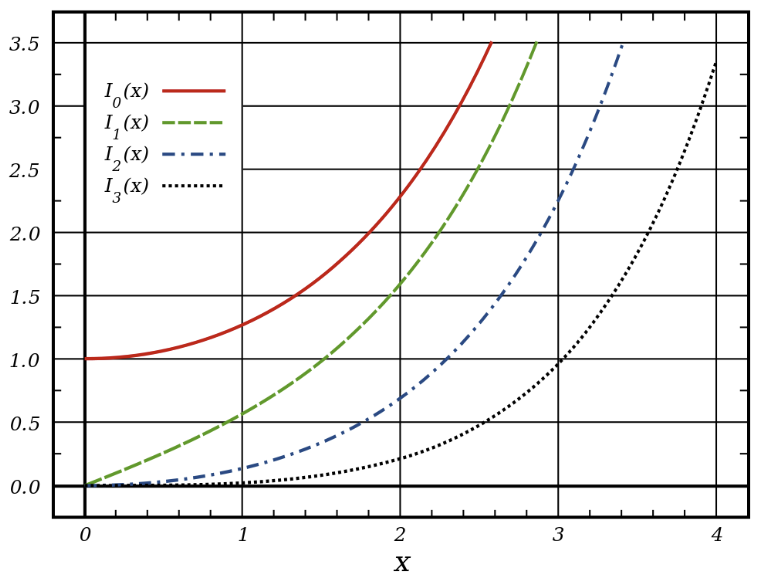
\includegraphics[width=7cm]{figures/I_nu.png}
    \caption{第一类虚宗量Bessel函数}
    \end{minipage}
    \begin{minipage}[t]{0.48\textwidth}
    \centering
    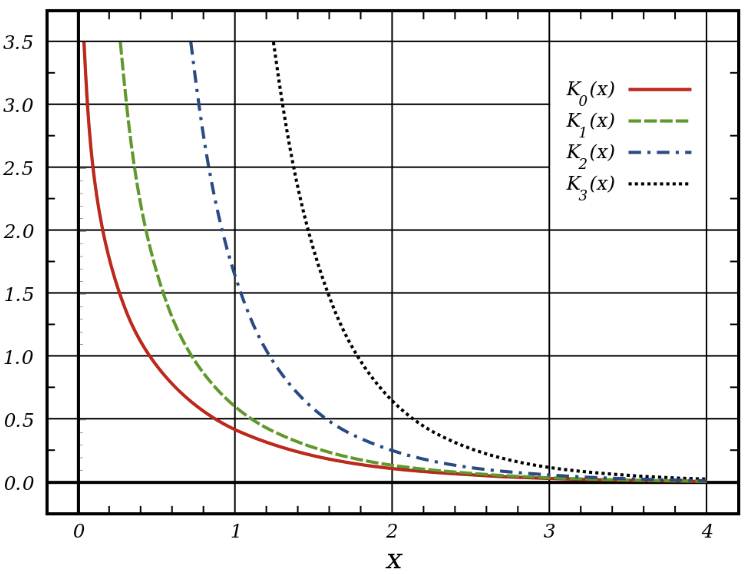
\includegraphics[width=7cm]{figures/K_nu.png}
    \caption{第二类虚宗量Bessel函数}
    \end{minipage}
\end{figure}
\noindent 1. 当$x\rightarrow\infty$时

$$\mathrm{I}_{\nu}(x)\sim\sqrt{\frac{1}{2\pi x}}\mathrm{e}^{x}\quad\mathrm{~K}_{\nu}(x)\thicksim\sqrt{\frac{\pi}{2x}}\mathrm{e}^{-x}$$

\noindent 2. 当$x\rightarrow0$时(约定$\nu\ge0$),$\mathrm{~I}_\nu(x)$有界,$\mathrm{~K}_\nu(x)$无界

\subsubsection{应用}
\begin{ex}[圆柱体Laplace方程]
$$\begin{aligned}
    &\nabla^{2}u=0\quad r<a,\quad0<z<h\\
    &u|_{\phi=0}=u|_{\phi=2\pi},\quad\frac{\partial u}{\partial\phi}\bigg|_{\phi=0}=\frac{\partial u}{\partial\phi}\bigg|_{\phi=2\pi}\\
    &u|_{r=0}<\infty,\quad u|_{r=a}=f(\phi,z)\\
    &u|_{z=0}=u|_{z=h}=0
\end{aligned}$$

\noindent 分离变量$u(r,\phi,z)=R(r)\Phi(\phi)Z(z)$

\noindent $\phi$方向:
$$\begin{cases}
    \Phi^{\prime\prime}+\lambda\Phi=0\\
    \Phi(0)=\Phi(2\pi),\Phi^{\prime}(0)=\Phi^{\prime}(2\pi)
\end{cases}\Rightarrow \lambda=m^2,\quad
\Phi_{m}=
\begin{cases}
    \cos m\phi&m=0,1,2\ldots\\
    \sin m\phi&m=1,2\ldots
\end{cases}$$

\noindent $z$方向:
$$\begin{cases}
    Z''+\lambda Z=0\\
    Z(0)=Z(h)=0
\end{cases}
\Rightarrow \lambda_{n}=(\frac{n\pi}{h})^{2}\quad n=1,2\dots\quad Z_{n}=\sin\frac{n\pi}{h}z
$$

\noindent $r$方向:
$$\frac{1}{r}\frac{d}{dr}(r\frac{dR}{dr})+(-\lambda-\frac{\mu}{r^{2}})R=0$$
$$\Rightarrow r\frac{d}{dr}(r\frac{dR}{dr})+[-(\frac{n\pi}{h}r)^{2}-m^{2}]R=0$$

变量代换:$x=\frac{n\pi}{h}r$
$$x\frac{d}{dx}(x\frac{dR}{dx})+[-x^{2}-m^{2}]R=0$$

得到$r$方向本征函数形式
$$\begin{aligned}R=&CI_{m}(x)+DK_{m}(x)\\=&I_{m}(\frac{n\pi}{h}r)\end{aligned}$$

\noindent 一般解形式
$$u=\sum_{m=0}^{\infty}\sum_{n=1}^{\infty}(A_{mn}\cos m\phi+B_{mn}\sin m\phi)I_{m}(\frac{n\pi}{h}r)\sin\frac{n\pi}{h}z$$

边界条件
$$u|_{r=a}=f(\phi,z)=\sum_{m=0}^{\infty}\sum_{n=1}^{\infty}(A_{mn}\cos m\phi+B_{mn}\sin m\phi)I_{m}(\frac{n\pi}{h}a)\sin\frac{n\pi}{h}z$$

利用正交性得
$$\begin{aligned}
    &A_{mn}I_{m}(\frac{n\pi}{h}a)=\frac{1}{\pi}\frac{1}{1+\delta_{m0}}\frac{2}{h}\int_{0}^{2\pi}d\phi\int_{0}^{h}dzf(\phi,z)\cos m\phi\sin\frac{n\pi}{h}z\\
    &B_{mn}I_{m}(\frac{n\pi}{h}a)=\frac{1}{\pi}\frac{2}{h}\int_{0}^{2\pi}d\phi\int_{0}^{h}dzf(\phi,z)\sin m\phi\sin\frac{n\pi}{h}z
\end{aligned}$$
\end{ex}

\subsection{球Bessel函数}
球坐标Helmholtz方程分离变量时,得到
$$\frac1{r^2}\frac{\mathrm{d}}{\mathrm{d}r}{\left(r^2\frac{\mathrm{d}R}{\mathrm{d}r}\right)}+\left(k^2-\frac\lambda{r^2}\right)R=0$$

在一般情况下,$$\lambda_l=l(l+1),l=0,1,2,\cdots $$

当$k=0$时,方程的解是$r^l$和$r^{-l-1}$

当$k\ne0$时:作变量代换$x=kr$,得
\begin{dfn}[球Bessel方程]
$$\frac{d}{dx}(x^{2}\frac{dR}{dx})+[x^{2}-l(l+1)]R=0$$
\end{dfn}

\noindent 可以将球Bessel方程化为$l+1$阶Bessel方程:

令$R(x)=\sqrt{\dfrac{\pi}{2x}}\nu(x)$
$$x\frac{d}{dx}(x\frac{dv}{dx})+[x^{2}-(l+\frac{1}{2})^{2}]\nu=0$$

\begin{dfn}[$l$阶球Bessel函数]
    $$\mathrm{j}_l(x)\equiv\sqrt{\frac\pi{2x}}\mathrm{J}_{l+1/2}(x)$$
\end{dfn}

\begin{dfn}[$l$阶球Neumann函数]
    $$\mathrm{n}_l(x)\equiv\sqrt{\frac{\pi}{2x}}\mathrm{N}_{l+1/2}(x)=(-1)^{l+1}\sqrt{\frac\pi{2x}}\mathrm{J}_{-(l+1/2)}(x)$$
\end{dfn}

\subsubsection{$j_l(x)$,$n_l(x)$的初等表达式} 
\noindent \textbf{0阶球Bessel和球Neumann函数}
$$\begin{aligned}
    J_{\frac{1}{2}}(x)=&\sum_{k=0}^{\infty}(-1)^{k}\frac{1}{k!\Gamma(k+\frac{3}{2})}\left(\frac{x}{2}\right)^{2k+\frac{1}{2}}\\
    =&\sum_{k=0}^{\infty}(-1)^{k}\frac{1}{(2k+1)!}x^{2k+\frac{1}{2}}\sqrt{\frac{2}{\pi}}
\end{aligned}$$

又有
$$\sin x=\sum_{k=0}^{\infty}\left(-1\right)^{k}\frac{1}{\left(2k+1\right)!}x^{2k+1}$$

因此
$$\begin{aligned}
    &J_{\frac{1}{2}}(x)=\sqrt{\frac{z}{\pi x}}\sin x\\
    &j_{0}(x)=\sqrt{\frac{\pi}{2x}}J_{\frac{1}{2}}(x)=\frac{1}{x}\sin x
\end{aligned}$$

$$\begin{aligned}
    &J_{-\frac{1}{2}}(x)=\sqrt{\frac{2}{\pi x}}\cos x=-N_{\frac{1}{2}}(x)\\
    &n_{0}(x)=-\frac{1}{x}\cos x 
\end{aligned}$$

\noindent \textbf{$l$阶球Neumann函数}

利用递推关系,
$$\begin{aligned}
    \frac{d}{dx}(x^{\nu}J_{\nu})=x^{\nu}J_{\nu-1}\quad\Rightarrow&\quad\frac{1}{x}\frac{d}{dx}(x^{\nu}J_{\nu})=x^{\nu-1}J_{\nu-1}\\
    (\frac{1}{x}\frac{d}{dx})^{l}(x^{\nu}J_{\nu})=&x^{\nu-l}J_{\nu-l}\\
    (\nu=-\frac{1}{2})\qquad(\frac{1}{x}\frac{d}{dx})^{l}(x^{-\frac{1}{2}}J_{-\frac{1}{2}})=&x^{-\frac{1}{2}-l}J_{-(l+\frac{1}{2})}\\
\end{aligned}$$
$$J_{-(l+\frac{1}{2})}(x)=\sqrt{\frac{2}{\pi}}x^{l+\frac{1}{2}}(\frac{1}{x}\frac{d}{dx})^{l}\left(\frac{\cos x}{x}\right)$$
$$\boxed{n_{l}(x)=(-1)^{l+1}x^{l}(\frac{l}{x}\frac{d}{dx})^{l}(\frac{\cos x}{x})}$$

例如
$$\mathrm{n}_0(x)=-\frac{\cos x}{x}\qquad\mathrm{n}_1(x)=-\frac{1}{x^2}\big(\cos x+x\sin x\big)$$
$$\mathrm{n}_2(x)=-\frac{1}{x^3}\Big[\left(3-x^2\right)\cos x+3x\sin x\Big]$$

\noindent \textbf{$l$阶球Bessel函数}

利用递推关系,
$$\begin{aligned}
    \frac{d}{dx}(x^{-\nu}J_{\nu})=-x^{-\nu}J_{\nu+\frac{1}{2}}\quad\Rightarrow&\quad\frac{1}{x}\frac{d}{dx}(x^{\nu}J_{\nu})=-x^{-(\nu+1)}J_{\nu+1}\\   
    (\frac{1}{x}\frac{d}{dx})^{l}(x^{-\nu}J_{\nu})=&(-1)^{l}x^{-(\nu+l)}J_{\nu+l}\\
    (\nu=\frac{1}{2})\qquad(\frac{1}{x}\frac{d}{dx})^{l}(x^{-\frac{1}{2}}J_{\frac{1}{2}})=&(-1)^{l}x^{-(l+\frac{1}{2})}J_{l+\frac{1}{2}}\\
\end{aligned}$$
$$J_{l+\frac{1}{2}}(x)=(-1)^{l}\sqrt{\frac{2}{\pi}}x^{l+\frac{1}{2}}(\frac{1}{x}\frac{d}{dx})^{l}(\frac{\sin x}{x})$$
$$\boxed{j_{l}(x)=\sqrt{\frac{\pi}{2x}}J_{l+\frac{1}{2}}=(-1)^{l}x^{l}(\frac{1}{x}\frac{d}{dx})^{l}(\frac{\sin x}{x})}$$

例如
$$\mathrm{j}_{0}(x)=\frac{\sin x}{x}\quad\mathrm{j}_{1}(x)=\frac{1}{x^{2}}\big(\sin x-x\cos x\big)$$
$$\mathrm{j}_{2}(x)=\frac{1}{x^{3}}\Big[\big(3-x^{2}\big)\sin x-3x\cos x\Big]$$
\subsubsection{渐进行为}

\begin{figure}[H]
    \centering 
    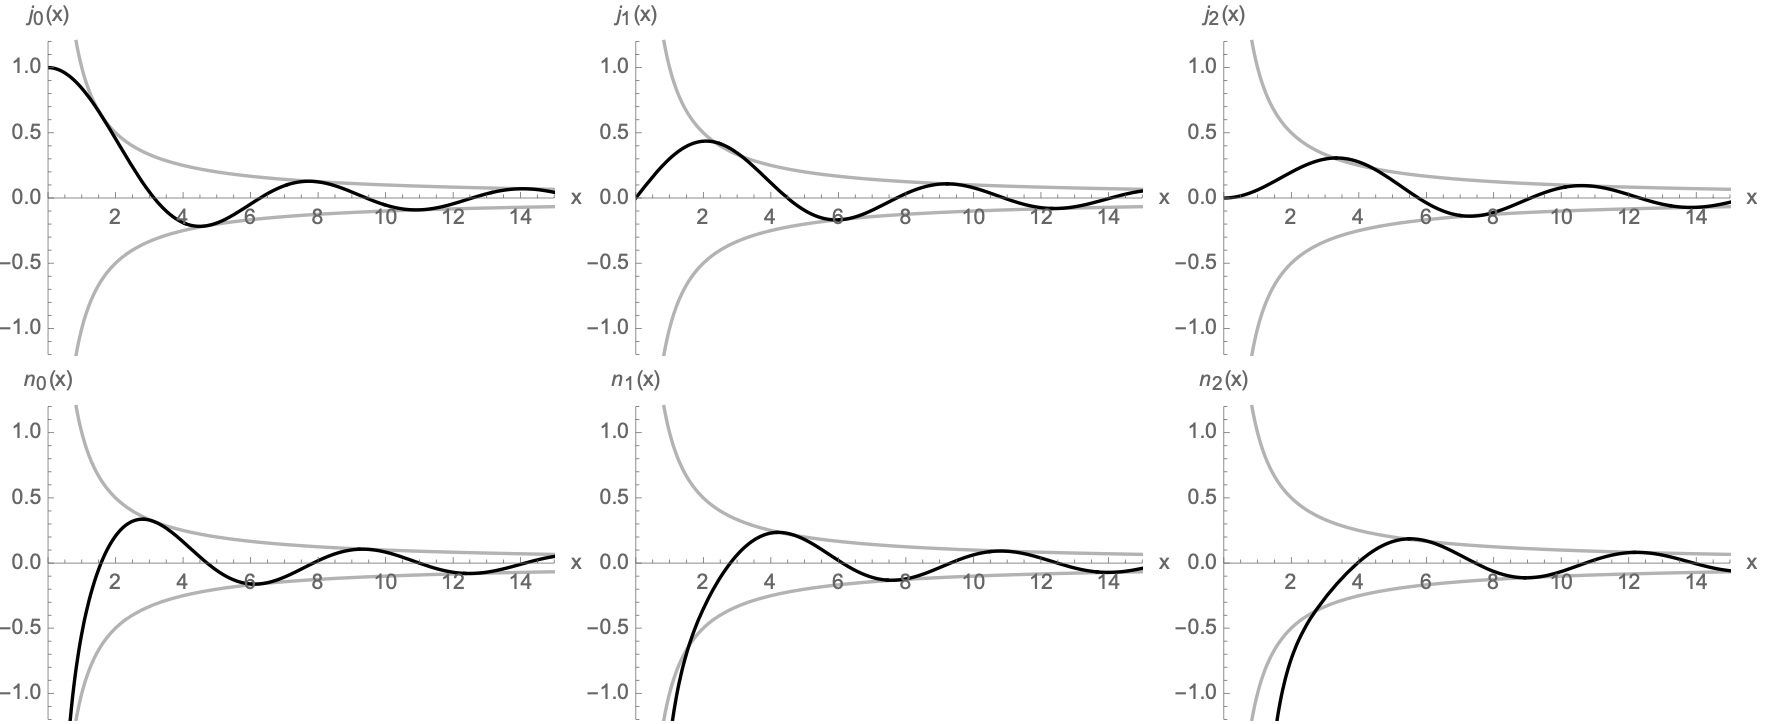
\includegraphics[width=15cm]{figures/SphereBessel.png} %插入图片,[]中设置图片大小,{}中是图片文件名
    \caption{球 Bessel 函数 $j_l(x)$ 和球 Neumann 函数 $n_l(x)$,其中细灰线为它们的渐进线$y=\pm\frac{1}{x}$} %最终文档中希望显示的图片标题
    \label{SphereBessel}
\end{figure}

$$\begin{aligned}
    x\to0:\quad &j_{0}(x)\to1,\quad j_{1}(x),j_{2}(x)\cdots\to0\\
    &n_{0}(x),n_{1}(x),n_{2}(x)\cdots\to\infty\\
    x\to\infty:\quad &j_{0},j_{1},j_{2},n_{0},n_{1},n_{2}\to0
\end{aligned}$$

\subsubsection{应用}
\begin{ex}[球内热传导问题]

    $$\frac{\partial u}{\partial t}=k\nabla^2u,\quad u|_{r=a}=0,\quad u|_{t=0}=f(r,\theta,\phi)$$

    $r$方向本征值问题:
$$\begin{cases}
\dfrac{1}{r^{2}}\dfrac{d}{dr}(r^{2}\dfrac{dR}{dr})+[\lambda-\dfrac{l(l+1)}{r^{2}}]R=0\\
R(0)<\infty,R(a)=0
\end{cases}$$

写成S-L标准形式,可见权函数$\rho(r)=r^2$
$$\frac{d}{dr}(r^{2}\frac{dR}{dr})+[\lambda r^{2}-l(l+1)]R=0$$

变量代换$x=\sqrt{\lambda}r$
$$\frac{d}{dx}(x^{2}\frac{dR}{dx})+[x^{2}-l(l+1)]R=0$$
$$R=j_{l}(x)=j_{l}(\sqrt{\lambda}r)$$

边界条件:
$$R(a)=0\Rightarrow j_{l}(\sqrt{\lambda}a)=0\Rightarrow\sqrt{\lambda_{n}}a=\mu_{n}^{(l)}$$
$$l=0:\quad j_{0}(x)=\frac{1}{x}\sin x\Rightarrow\quad\mu_{n}^{(0)}=n\pi,\quad n=1,2,3\ldots $$

广义傅里叶级数:
$$\begin{aligned}
    [0,a]&=f(r)=\sum_{n=1}^{\infty}c_{n}j_{l}(\frac{\mu_{n}^{(l)}}{a}r)\\
    C_{n}&=\frac{1}{||j_{l}(\frac{\mu_{n}^{(l)}}{a}r)||^{2}}\int_{0}^{a}f(r)j_{l}(\frac{\mu_{n}^{(l)}}{a}r)r^{2}dr
\end{aligned}$$
\end{ex}